% gm-01-sets.tex

\documentclass[xcolor=dvipsnames]{beamer}

\usepackage{cancel}
\renewcommand{\CancelColor}{\color{red}}
\usepackage{graphicx}
\usepackage{wrapfig}
\usepackage{colortbl}
\usepackage{color}
\usepackage{alltt}
\renewcommand*{\thefootnote}{\fnsymbol{footnote}}
\definecolor{myblue}{rgb}{0.8,0.85,1}

\mode<presentation>
{
  \usetheme{Warsaw}
  \setbeamercovered{transparent}
}
% \usecolortheme[named=OliveGreen]{structure}
\setbeamertemplate{navigation symbols}{} 
\setbeamertemplate{blocks}[rounded][shadow=true] 

% this is for overlaying math symbols, see https://tex.stackexchange.com/questions/12895/overlay-symbol-with-another
\def\qeq{\mathrel{%
    \mathchoice{\QEQ}{\QEQ}{\scriptsize\QEQ}{\tiny\QEQ}%
}}
\def\QEQ{{%
    \setbox0\hbox{$\longrightarrow$}%
    \rlap{\hbox to \wd0{\hss/\hss}}\box0
  }}

\newcounter{expls}
\setcounter{expls}{0}
\newcommand{\beispiel}[1]{\refstepcounter{expls}\textbf{Example \arabic{expls}: #1.}}

\newcounter{exercise}
\setcounter{exercise}{0}
\newcommand{\ubung}[0]{\refstepcounter{exercise}\textbf{Exercise \arabic{exercise}: }}

\newif\ifBCITCourse
\BCITCoursetrue
% \BCITCoursefalse
\newif\ifWhichCourse
\WhichCoursetrue
\WhichCoursefalse
\ifBCITCourse
\ifWhichCourse
\newcommand{\CourseName}{Technical Mathematics for Food Technology}
\newcommand{\CourseNumber}{MATH 1441}
\newcommand{\CourseInst}{BCIT}
\else
\newcommand{\CourseName}{Technical Mathematics for Geomatics}
\newcommand{\CourseNumber}{MATH 1511}
\newcommand{\CourseInst}{BCIT}
\fi
\else
\newcommand{\CourseName}{Philosophy and Literature}
\newcommand{\CourseNumber}{PHIL 375}
\newcommand{\CourseInst}{UBC}
\fi

\title{Set Theory, Functions, Numbers}
\subtitle{{\CourseNumber}, BCIT}

\author{\CourseName}

\date{September 7, 2017}

\begin{document}

\begin{frame}
  \titlepage
\end{frame}

\begin{frame}
  \frametitle{Sets}
  A \alert{set} is a rule: for each object, the rule tells you
  unambiguously whether the object belongs to the set or not. We say
\begin{equation}
  \label{eq:ohkaifoh}
  x\in{}A
\end{equation}
when an object $x$ belongs to a set $A$. When it does not belong to
set $A$ we say
\begin{equation}
  \label{eq:naeseich}
  x\notin{}A
\end{equation}

Statements like (\ref{eq:ohkaifoh}) or (\ref{eq:naeseich}) are called
\alert{propositions}. They are either true or false. Logic is ``under
the hood'' for the vehicle that is set theory. Set theory is ``under
the hood'' for the vehicle that is mathematics.
\end{frame}

\begin{frame}
  \frametitle{Sets}
There are many different ways to write out the rules whether an object
belongs to a set or not. One is to just list the objects in curly
braces, such as
\begin{equation}
  \label{eq:eichaewi}
  S=\{\clubsuit,\spadesuit,\diamondsuit,\heartsuit\}
\end{equation}
Rule (\ref{eq:eichaewi}) tells us that no object belongs to set $B$
except these four: $\clubsuit,\spadesuit,\diamondsuit,\heartsuit$.
They are the \alert{elements} of $S$. Order does not matter. There is
one very special set: the \alert{empty set} $\emptyset$. The rule for
the empty set is that no object belongs to it. It is sometimes written
$\{\}$.
\end{frame}

\begin{frame}
  \frametitle{Set Operators}
  Sets can relate to each other in certain ways. For example,
  \begin{equation}
    \label{eq:johbaexi}
    \{\clubsuit,\diamondsuit\}\subset\{\clubsuit,\spadesuit,\diamondsuit,\heartsuit\}
  \end{equation}
  $A\subset{}B$ ($A$ is a \alert{subset} of $B$) if and only if all
  elements of $A$ are also elements of $B$. Two sets are equal if and
  only if $A\subset{}B$ and $B\subset{}A$. We say $A=B$. If they are
  not equal, we say $A\neq{}B$. $B\supset{}A$ means the same as
  $A\subset{}B$, but we usually say that $B$ is a superset of $A$.
\end{frame}

\begin{frame}
  \frametitle{Set Operators}
  If $A\subset{}X$, then the complement of $A$ with respect to $X$ is
  the set of objects that belong to $X$ but not to $A$. We say $A^{C}$
  or $\bar{A}$, and often $X$ as the \alert{universal set} is not
  mentioned explicitly.

  For two sets $A$ and $B$, set subtraction gives us $A-B$ or
  $A\setminus{}B$, which contains all elements in $A$ which are not in
  $B$. If $A\subset{}X$ then
  \begin{equation}
    \label{eq:sogaebae}
    X\setminus{}A=A^{C}
  \end{equation}
\end{frame}

\begin{frame}
  \frametitle{Unions and Intersections}
  The \alert{union} of two sets $A$ and $B$ is the group of objects $x$ for
  which it is true that $x\in{}A$ or $x\in{}B$. We say
  \begin{equation}
    \label{eq:atohzohb}
    A\cup{}B
  \end{equation}

  The \alert{intersection} of two sets $A$ and $B$ is the group of objects $x$ for
  which it is true that $x\in{}A$ and $x\in{}B$. We say
  \begin{equation}
    \label{eq:yeerahte}
    A\cap{}B
  \end{equation}

  Two sets $A$ and $B$ are \alert{disjoint} if they have no elements in
  common, i.e.\ $A\cap{}B=\emptyset$.
\end{frame}

\begin{frame}
  \frametitle{Russell's Paradox}
  Sets can be elements of sets. The following set has three elements.
  \begin{equation}
    \label{eq:ginoicoo}
A=\{\{\clubsuit,\heartsuit\},\{\},\{\heartsuit,\spadesuit,\diamondsuit\}\}    
  \end{equation}
  How many elements does this set have?
  \begin{equation}
    \label{eq:phuileob}
    B=\{\{\{\{\{\{\{\}\}\}\}\}\}\}
  \end{equation}
The father of set theory, Gottlob Frege, thought that all sets make
sense as long as they are well-defined. Another famous mathematician,
Bertrand Russell, figured out that that was not quite right. Think of
the set $R$ that contains all sets which do not contain themselves
(some sets do contain themselves, for example the set of all
non-lemons). Does $R$ contain itself?
\end{frame}

\begin{frame}
  \frametitle{Natural Numbers}
On the previous slide, I said that a set had three elements. The point
of set theory is to give a foundation for numbers, not the other way
around. So I jumped the gun. We don't know yet what ``three'' means.
To avoid Russell's paradox, let's restrict ourselves to sets that do
not contain themselves. Then we define the successor $A^{+}$ of a set $A$ to
be the following
\begin{equation}
  \label{eq:mooxeefi}
  A^{+}=A\cup\{A\}
\end{equation}
Note that $A$ does not contain itself and $A^{+}$ does not contain
itself. 
\end{frame}

\begin{frame}
  \frametitle{Natural Numbers}
  Now we give names to the following sets:

  \bigskip

\begin{tabular}{rclcl}
    $\emptyset$ & \hspace{.5in} & ``zero'' & \hspace{.5in} & 0 \\ 
    $\emptyset^{+}$ & \hspace{.5in} & ``one'' & \hspace{.5in} & 1 \\ 
    $\displaystyle \left(\emptyset^{+}\right)^{+}$ & \hspace{.5in} & ``two'' & \hspace{.5in} & 2 \\ 
    $\displaystyle \left(\left(\emptyset^{+}\right)^{+}\right)^{+}$ & \hspace{.5in} & ``three'' & \hspace{.5in} & 3 \\ 
  \end{tabular}

\bigskip

  and so on. The set of all these sets is $\mathbb{N}$, the natural
  numbers.

  {\ubung} Write the set 3 using curly braces.
\end{frame}

\begin{frame}
  \frametitle{Natural Numbers}
Another way to write a rule for a set is to use pattern
  matching
  \begin{equation}
    \label{eq:aiheegor}
    \mathbb{N}=\{0,1,2,3,\ldots\}
  \end{equation}
  For example, the set of odd numbers is
  \begin{equation}
    \label{eq:laibaesh}
 \mathbb{N}_{\mbox{\tiny odd}}=\{1,3,5,7,\ldots\}
  \end{equation}
\end{frame}

\begin{frame}
  \frametitle{Ordered Pairs}
  An ordered pair is a set which determines an order in which the
  components of an ordered pair can be read. Let $G=\{a,b\}$. Then
  the collection of ordered pairs in $G$ (we call this collection the
  set $G\times{}G$)
  \begin{equation}
    \label{eq:aijeenge}
   G\times{}G=\{(a,a),(a,b),(b,a),(b,b)\}
  \end{equation}
$(a,b)$ and the other elements of this set are \alert{ordered pairs}.
They are defined as follows:
\begin{equation}
  \label{eq:phohpahj}
  (a,b)=\{\{a\},\{a,b\}\}
\end{equation}
Notice that even though $\{a,b\}=\{b,a\}$ (order does not matter for
sets), $(a,b)\neq(b,a)$ (order matters for ordered pairs). Coordinates
are an example of ordered pairs (or ordered triplets, and so on).
\end{frame}

\begin{frame}
  \frametitle{Functions}
The \alert{set product} is best explained by example. Let $A=\{a_{1},a_{2},a_{3}\}$ and
$W=\{w_{1},w_{2}\}$. Then
\begin{equation}
  \label{eq:oochohdi}
  A\times{}W=\{(a_{1},w_{1}),(a_{1},w_{2}),(a_{2},w_{1}),(a_{2},w_{2}),(a_{3},w_{1}),(a_{3},w_{2})\}\notag
\end{equation}
The elements of $A\times{}W$ are ordered pairs.
% ; they are
% strange sets where the order matters (one way to define them as sets
% is to say that $(a_{1},w_{1})=\{\{a_{1}\},\{a_{1},w_{1}\}\}$).
A \alert{function} $f:A\rightarrow{}W$ is a subset of $A\times{}W$ with the
following rule (we will write $f(a)=w$ instead of $(a,w)\in{}f$ to
make it more readable):
\begin{quote}
For each element in $a\in{}A$, there must be exactly one ordered pair in $f$
  such that $f(a)=w$ ($w\in{}W$).
\end{quote}
\end{frame}

\begin{frame}
  \frametitle{Functions}
  If $f:A\rightarrow{}W$ is a function, then $A$ is the \alert{domain}
  and $W$ is the \alert{codomain}. Those $w$ in $W$ for which $f(a)=w$
  form a subset of $W$ called the \alert{range} of the function.

  \bigskip

  If $f(a)=w$ and $f(b)=w$ implies that $a=b$ ($a=b$ means that there
  is one and the same object with two labels $a$ and $b$), then $f$ is
  called \alert{one-to-one} or \alert{injective}. If the codomain is a
  subset of the range, then $f$ is called \alert{onto} or
  \alert{surjective}. If a function is both injective and surjective,
  then it is called \alert{bijective}.
\end{frame}

\begin{frame}
  \frametitle{Function Graphs}
  A \alert{function graph} is just another rule for a set.
  \alert{Points} in the $xy$-plane are elements of
  $\mathbb{R}\times\mathbb{R}$, sometimes called $\mathbb{R}^{2}$. The
  function graph identifies all those points which form the set
  \begin{equation}
    \label{eq:oongaiku}
    f=\{(x,y)|P=(x,y)\mbox{ and }P\mbox{ is on the function graph}\}
  \end{equation}
Therefore $f\subset\mathbb{R}^{2}$ and if each $x\in\mathbb{R}$ is
associated with a unique element $y\in\mathbb{R}$, then $f$ is a
function. Many subsets of $\mathbb{R}^{2}$ are not functions. If
$P=(x,y)$ is on the function graph the following two statements have
the same meaning:
\begin{equation}
  \label{eq:aipeejae}
  y=f(x)
\end{equation}
\begin{equation}
  \label{eq:aecaekax}
  (x,y)\in{}f
\end{equation}
\end{frame}

\begin{frame}
  \frametitle{Injective and Surjective Functions}
  \begin{figure}[h]
    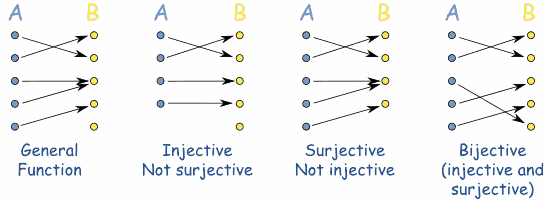
\includegraphics[scale=0.6]{./function-mapping.png}
  \end{figure}
\end{frame}

\begin{frame}
  \frametitle{Cardinality}
If there is a bijective function $f:A\rightarrow{}B$ for two sets $A$
and $B$, then $A$ and $B$ share the same cardinality $n(A)=n(B)$.
If there is a bijective function from any set $B$ to a set in
$\mathbb{N}$, then that element of $\mathbb{N}$ is the cardinality of
$B$. In other words, since there is a  bijective function from 3 to
\begin{equation}
  \label{eq:ohriohar}
  B=\{\clubsuit,\heartsuit,\diamondsuit\}
\end{equation}
the cardinality of $B$ is three. Not all cardinalities are natural
numbers, for example $n(\mathbb{N})$.
\end{frame}

\begin{frame}
  \frametitle{Integers and Fractions}
  We use more set theory to define the integers:
  \begin{equation}
    \label{eq:eofiebee}
    \mathbb{Z}=\{\ldots,-2,-1,0,1,2,3,\ldots\}
  \end{equation}
  Then we use a similar strategy to define the rational numbers:
  \begin{equation}
    \label{eq:ciuceeke}
    \mathbb{Q}=\left\{\ldots,-\frac{14}{17},\ldots,-\frac{1}{2},\ldots,0,\ldots,\frac{1}{7},\ldots,4,\ldots,\frac{19}{4},\ldots\right\}\notag
  \end{equation}
  For the definition of $\mathbb{Z}$ and $\mathbb{Q}$ we need a
  concept of set theory called \alert{equivalence relation}. For the
  definition of operators such as $+,-,\cdot,\div$ and exponents we
  need a concept of set theory called \alert{induction}. We will not
  cover these two concepts in this brief introduction and rely on our
  intuition instead.
\end{frame}

\begin{frame}
  \frametitle{Hippasus of Metapontum}
It turns out that $\mathbb{N}$,$\mathbb{Z}$, and $\mathbb{Q}$ have the
same cardinality. A Greek mathematician called Hippasus
figured out that the square root of 2 is not an element of any of
these sets. You can duckduckgo the proof for this fact. It is not
difficult to understand; it uses prime numbers.
\end{frame}

\begin{frame}
  \frametitle{Hippasus of Metapontum}
  \begin{figure}[h]
    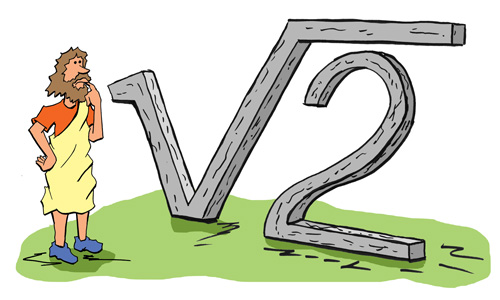
\includegraphics[scale=0.6]{./hippasusofmetapontum.jpg}
  \end{figure}
\end{frame}

\begin{frame}
  \frametitle{Terrible Twos}
  \begin{figure}[h]
    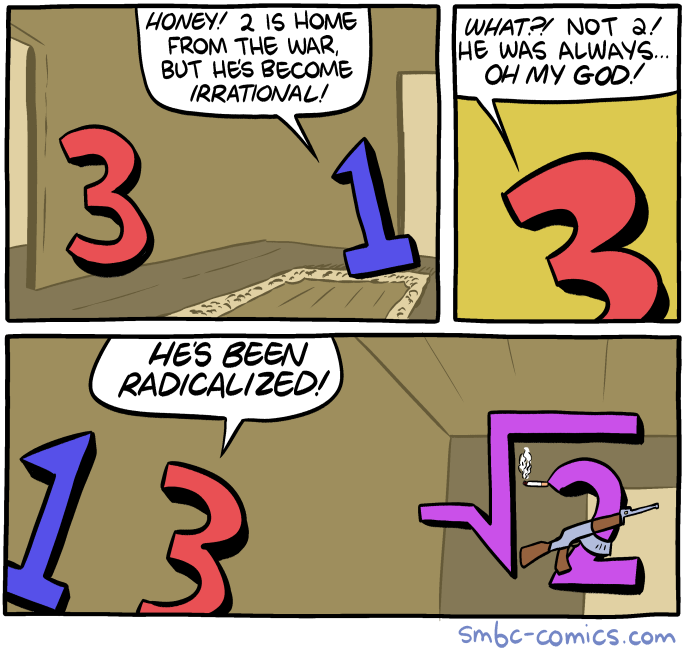
\includegraphics[scale=0.35]{./radicalized.png}
  \end{figure}
\end{frame}

\begin{frame}
  \frametitle{The Real Numbers}
Some more complicated math is necessary to construct the real number
line, including such irrational numbers as $\sqrt{2},\pi,$ and $e$. We
call the set of real numbers $\mathbb{R}$. Make sure to remember that
\begin{equation}
  \label{eq:ainieroo}
  \mathbb{N}\subset\mathbb{Z}\subset\mathbb{Q}\subset\mathbb{R}
\end{equation}
However, the cardinality of $\mathbb{R}$ is not the same as the
cardinality of $\mathbb{Q}$. Again, you can duckduckgo the proof, which is
not difficult to understand; it uses Cantor's diagonal argument. It is
a very difficult question (unresolved as far as I know) whether there
is a set that has more elements than $\mathbb{N}$ and fewer elements
than $\mathbb{R}$.
\end{frame}

\begin{frame}
  \frametitle{Power Sets and Interval Notation}
  The \alert{power set} of a set $A$ is the set which contains all the
  subsets of $A$ (it always contains $A$ and $\emptyset$). It is
  sometimes called $\mathfrak{p}(A)$. The cardinality of
  $\mathfrak{p}(\mathbb{N})$ is the same as the cardinality of
  $\mathbb{R}$.

  Another way to write a rule for a set is as follows:
  \begin{equation}
    \label{eq:oosaeshu}
    [-7,2)=\{x\in\mathbb{R}|-7\leq{}x\mbox{ and }x<2\}
  \end{equation}

  The infinity sign $\infty$ is used when there is no boundary on the
  left or the right of the number line:
  \begin{equation}
    \label{eq:susheipe}
    \left.\left(-\infty,\frac{1}{2}\right.\right]=\left\{x\in\mathbb{R}|x\leq\frac{1}{2}\right\}
  \end{equation}
\end{frame}

\begin{frame}
  \frametitle{Equations}
  Equations are rules for sets. The equation $2x=6$ is a rule for the set
  \begin{equation}
    \label{eq:vaechohd}
    S=\{x\in\mathbb{R}|2x=6\}
  \end{equation}
  The two rules $2x=6$ and $5-x=2$ yield the same set. We say that
  these two equations are \alert{equivalent}. Note that the solution
  set is assumed to be a subset of $\mathbb{R}$.
  \begin{equation}
    \label{eq:xeedoogh}
    S_{\mathbb{R}}=\{x\in\mathbb{R}|x^{2}=-1\}=\{\}
  \end{equation}
  \begin{equation}
    \label{eq:aidietha}
    S_{\mathbb{C}}=\{x\in\mathbb{C}|x^{2}=-1\}=\{i,-i\}
  \end{equation}
\end{frame}

\begin{frame}
  \frametitle{Manipulating Equations}
  Solving an equation often means listing the elements of its
  \alert{solution set} in curly
  braces, for example
  \begin{equation}
    \label{eq:ohnomoow}
    S=\{x\in\mathbb{R}|2x=6\}=\{3\}
  \end{equation}
If we apply a bijective function to both sides of the equation, the
original and the resulting equation are equivalent. Let $F$ be a
bijective function $F:\mathbb{R}\rightarrow\mathbb{R}$. We usually use
linear functions $F$ for this purpose. Then
\begin{equation}
  \label{eq:iikucire}
  \{x\in\mathbb{R}|2x=6\}=\{x\in\mathbb{R}|F(2x)=F(6)\}
\end{equation}
{\ubung} Use the function $F(X)=\frac{1}{2}\cdot{}X$ to find the equivalent
equation to $2x=6$.
\end{frame}

\begin{frame}
  \frametitle{Venn Diagrams}
  Sometimes we use Venn diagrams to define or clarify the composition
  of various sets.
  \begin{figure}[h]
    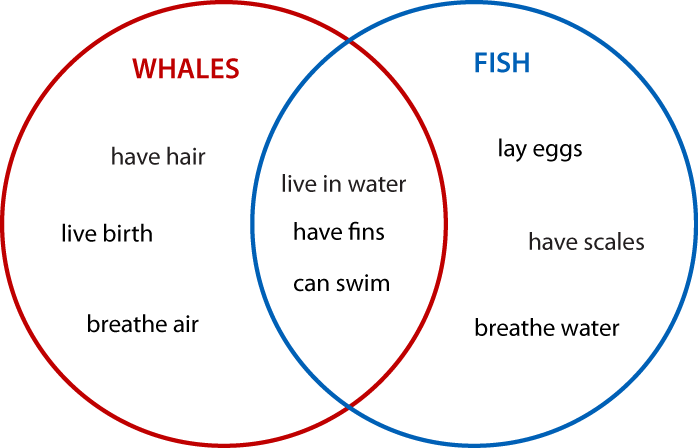
\includegraphics[scale=0.7]{./animals-01.png}
  \end{figure}
\end{frame}

\begin{frame}
  \frametitle{End of Lesson}
Next Lesson: Linear Equations
\end{frame}

\end{document}

hhhh